\section{Results and Discussion}
This section presents the results of the system,
and discusses the results.

\subsection{Results}
The results of the system can be seen in the web
application.

The system successfully gathers the data from the
MQ135 and DHT22 sensors, and displays the data in
the web application.
% as seen in \ref{webapp-stats-view}.
The system successfully open and close the door by
determining the current average of the indicators,
and act accordingly.

As seen in \ref{webapp-home-view}, the web application
could be used as the interface to control the system,
changing system mode, and opening and closing the door
remotely.

\begin{figure}
      \centerline{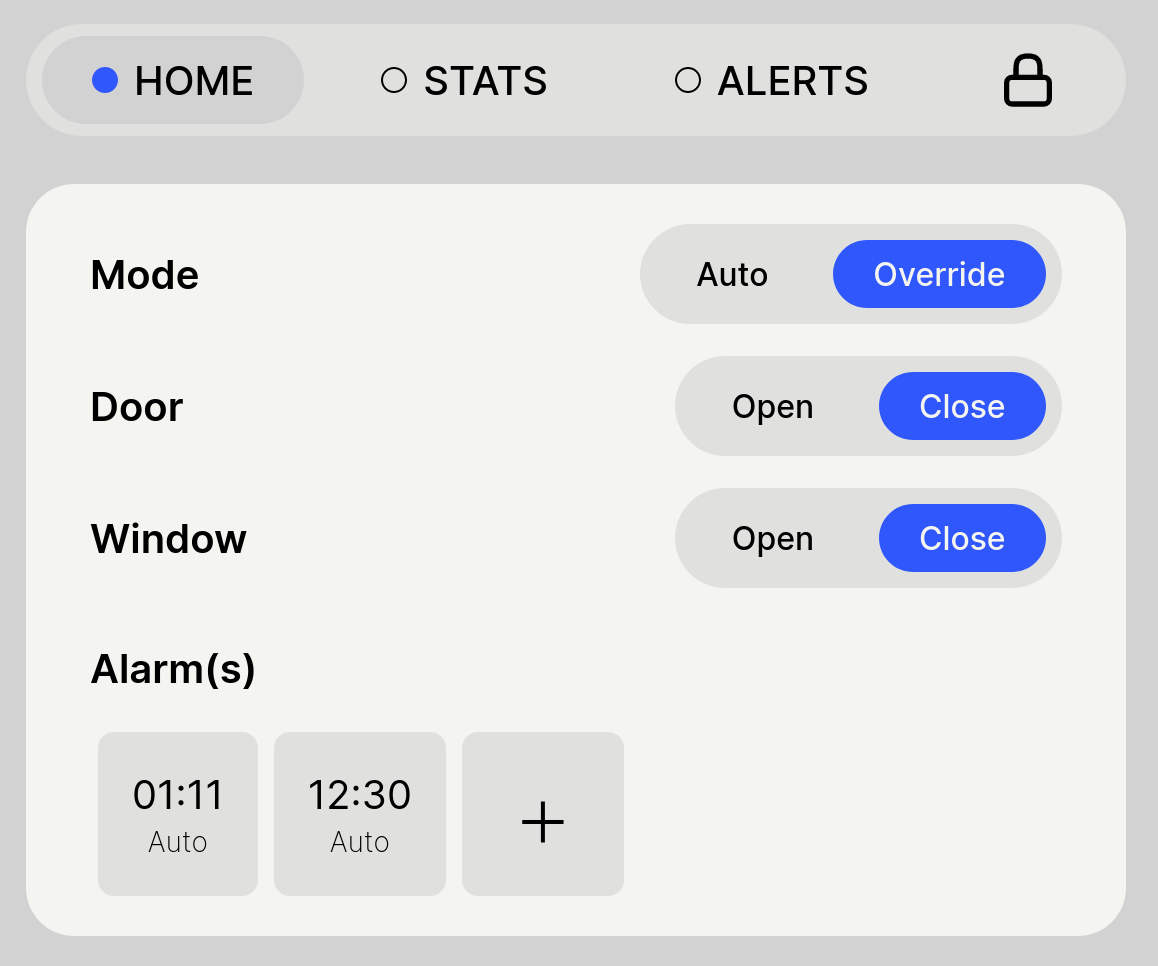
\includegraphics[scale=0.2]{resources/webapp-home-view.png}}
      \caption{Home view of the web application of the smart room air conditioner}
      \label{webapp-home-view}
\end{figure}

\textcolor{red}{
      \textbf{
            \emph{TODO: add more detail and/
                  or screenshot of the web application.}
      }
}

\subsection{Discussion}
\subsubsection{Sensors}
The sensors used in the system could detect the
indicators of the air quality, but the accuracy
of the sensors are still questionable.
Specifically, the MQ135 sensor, which is used to
detect the carbon dioxide (CO2) ppm, is not
accurate enough to be used as a reference for.
The MQ135 sensor's base resistance (RZERO) is
not stable, thus affecting the sensor's
reading of the CO2 ppm.

\subsubsection{Machine Learning}
Although the system could already determine to open
or close the door, the system is still far from
perfect. The decision making of opening and closing
the door is merely based on the data from the
sensors and the clustering model. While the actual
air quality of the room related to the health,
comfort, and productivity of the inhabitant are not
considered.

\subsubsection{System Architecture}
Other issues is that, architeturally, the machine
learning model is deployed in the same server with
the application backend, thus lowering the
performance of the application backend, when the
machine learning model is being used.
